% FSB Seminar — Sveučilište u Zagrebu, Fakultet strojarstva i brodogradnje
% Template v2.1 — latex_architect popunjava placeholdere iz project.yaml
% Project adaptations (PAS-DUAL-ARM): three course instructors on the title page,
% GitHub page after the title page, listings/TikZ/siunitx, figure macros with a
% placeholder box (\slika, \dvijeslike), list of listings, appendices.

\documentclass[12pt,a4paper]{article}

% --- Encoding, Font & Language (dual-engine) ---
% Kanonski engine je Tectonic (XeTeX): fontspec + TeX Gyre Termes ima PRAVI
% OpenType bold pa hrvatski ž/ć/š/đ rade i u \textbf{}. pdfLaTeX fallback koristi
% newtxtext (vidi gotcha miktex-t1-bold-diacritics). NE newtxmath uz amssymb (\Bbbk konflikt).
% Monospace: Inconsolata (has a real bold, needed for keywords in code listings).
\usepackage{iftex}
\ifPDFTeX
  \usepackage[utf8]{inputenc}
  \usepackage[T1]{fontenc}
  \usepackage{newtxtext}
  \usepackage[varqu]{zi4}
\else
  \usepackage{fontspec}
  \setmainfont{texgyretermes-regular.otf}[
    BoldFont       = texgyretermes-bold.otf,
    ItalicFont     = texgyretermes-italic.otf,
    BoldItalicFont = texgyretermes-bolditalic.otf
  ]
  \setmonofont{Inconsolatazi4-Regular.otf}[
    BoldFont = Inconsolatazi4-Bold.otf,
    Scale    = MatchLowercase
  ]
\fi
\usepackage[croatian]{babel}

% --- Layout ---
\usepackage[top=2.5cm,bottom=2.5cm,left=2.5cm,right=2.5cm]{geometry}
\usepackage{setspace}
\onehalfspacing

% --- Headers & Footers ---
\usepackage{fancyhdr}
\setlength{\headheight}{13.6pt}
\pagestyle{fancy}
\fancyhf{}
\fancyhead[L]{\small\itshape \authorname}
\fancyhead[R]{\small\itshape \seminartitleshort}
\fancyfoot[L]{\small\itshape Fakultet strojarstva i brodogradnje}
\fancyfoot[R]{\small\itshape\thepage}
\renewcommand{\headrulewidth}{0.4pt}
\renewcommand{\footrulewidth}{0.4pt}

% --- Section Formatting (14pt Bold Uppercase) ---
\usepackage{titlesec}
\titleformat{\section}
  {\normalfont\fontsize{14}{17}\bfseries\MakeUppercase}
  {\thesection.}{0.5em}{}
\titleformat{\subsection}
  {\normalfont\fontsize{12}{15}\bfseries}
  {\thesubsection.}{0.5em}{}
\titleformat{\subsubsection}
  {\normalfont\fontsize{12}{15}\bfseries\itshape}
  {\thesubsubsection.}{0.5em}{}
\titleformat{\paragraph}[runin]
  {\normalfont\fontsize{12}{15}\itshape}
  {}{0em}{}[.]

% --- Figures & Tables ---
\usepackage{graphicx}
\graphicspath{{figures/}}
\usepackage{booktabs}
\usepackage{tabularx}
\usepackage{longtable}
\usepackage{array}
\usepackage{float}
\usepackage{caption}
\captionsetup[figure]{font={small,bf},labelsep=period,position=below}
\captionsetup[table]{font={small,bf},labelsep=period,position=above}
\usepackage{subcaption}
\captionsetup[subfigure]{font=small,labelformat=parens,labelsep=space}
\usepackage{pdflscape}   % \begin{landscape} ... \end{landscape} for wide figures/tables

% --- Figure/Table numbering by section (Slika 2.1, Tablica 2.1) ---
\usepackage{chngcntr}
\counterwithin{figure}{section}
\counterwithin{table}{section}
\counterwithin{equation}{section}

% --- Depth ---
\setcounter{secnumdepth}{4}
\setcounter{tocdepth}{4}

% --- Croatian names (addto — babel croatian overrida renewcommand) ---
\addto\captionscroatian{%
  \renewcommand{\figurename}{Slika}%
  \renewcommand{\tablename}{Tablica}%
  \renewcommand{\contentsname}{\normalfont\fontsize{14}{17}\bfseries SADRŽAJ}%
  \renewcommand{\listfigurename}{\normalfont\fontsize{14}{17}\bfseries POPIS SLIKA}%
  \renewcommand{\listtablename}{\normalfont\fontsize{14}{17}\bfseries POPIS TABLICA}%
  \renewcommand{\refname}{\normalfont\fontsize{14}{17}\bfseries LITERATURA}%
}

% --- References ---
\usepackage{cite}

% --- Hyperlinks ---
\usepackage[hidelinks,unicode]{hyperref}

% --- Math ---
\usepackage{amsmath}
\usepackage{amssymb}

% --- Color (za upozorenja o nepopunjenim placeholderima) ---
\usepackage{xcolor}

% --- Units: \SI{0.30}{\metre}, \num{1.5} -> decimal comma ---
\usepackage{siunitx}
\sisetup{output-decimal-marker={,}}

% --- Diagrams (architecture, launch hierarchy, state machines) ---
\usepackage{tikz}
\usetikzlibrary{positioning, arrows.meta, shapes.geometric, fit, backgrounds, calc}

% ============================================================
% CODE LISTINGS
% ============================================================
% Usage:
%   \begin{lstlisting}[style=code-python, caption={...}, label={lst:...}]
%   ...
%   \end{lstlisting}
%   \lstinputlisting[style=code-yaml, firstline=10, lastline=30,
%                    caption={...}, label={lst:...}]{code/controllers.yaml}
% Styles:    code (base, default for every listing), code-python, code-xml,
%            code-yaml, code-bash
% Languages: Python, XML, bash (built into listings), yaml (defined below)
% Captions read "Ispis <section>.<n>." and appear in "POPIS ISPISA".
\usepackage{listings}

\lstdefinelanguage{yaml}{
  keywords={true, false, null, True, False},
  sensitive=false,
  comment=[l]{\#},
  morestring=[b]',
  morestring=[b]"
}

\lstdefinestyle{code}{
  basicstyle=\footnotesize\ttfamily\setstretch{1},
  keywordstyle=\color{blue!60!black}\bfseries,
  commentstyle=\color{green!40!black},
  stringstyle=\color{red!55!black},
  numbers=left,
  numberstyle=\tiny\color{gray},
  numbersep=6pt,
  frame=single,
  rulecolor=\color{gray!60},
  backgroundcolor=\color{gray!6},
  framesep=3pt,
  framexleftmargin=16pt,
  xleftmargin=20pt,
  xrightmargin=4pt,
  breaklines=true,
  breakatwhitespace=false,
  postbreak=\mbox{\textcolor{gray}{$\hookrightarrow$}\space},
  columns=fullflexible,
  keepspaces=true,
  showstringspaces=false,
  tabsize=4,
  upquote=true,
  captionpos=t,
  aboveskip=\medskipamount,
  belowskip=\medskipamount,
  extendedchars=true
}

% Croatian letters inside listings.
% pdfLaTeX: multi-byte UTF-8 input needs `literate` replacements.
% XeTeX/LuaTeX (Tectonic): listings only puts characters 0-255 into its char
% table, so letters such as č (U+010D) bypass it and get typeset out of order
% ("ačb" -> "čab") and without the comment/string colour; `literate` does not
% help there. Registering them as letters in the char table fixes both.
\makeatletter
\ifPDFTeX
  \lstset{literate={č}{{\v{c}}}1 {ć}{{\'c}}1 {ž}{{\v{z}}}1 {š}{{\v{s}}}1 {đ}{{\dj}}1
                   {Č}{{\v{C}}}1 {Ć}{{\'C}}1 {Ž}{{\v{Z}}}1 {Š}{{\v{S}}}1 {Đ}{{\DJ}}1}
\else
  \def\pas@lstUnicodeLetter#1{%
    \lst@ifactivechars\catcode`#1=\active\fi
    \begingroup\lccode`\~=`#1\lccode`\/=`#1%
    \lowercase{\endgroup\def~{\lst@ProcessLetter/}}}
  \lst@AddToHook{SelectCharTable}{%
    \pas@lstUnicodeLetter č\pas@lstUnicodeLetter ć\pas@lstUnicodeLetter ž%
    \pas@lstUnicodeLetter š\pas@lstUnicodeLetter đ\pas@lstUnicodeLetter Č%
    \pas@lstUnicodeLetter Ć\pas@lstUnicodeLetter Ž\pas@lstUnicodeLetter Š%
    \pas@lstUnicodeLetter Đ}
\fi
\makeatother

\lstdefinestyle{code-python}{
  style=code,
  language=Python,
  morekeywords={as, assert, async, await, nonlocal, with, yield, True, False, None}
}
\lstdefinestyle{code-xml}{
  style=code,
  language=XML,
  tagstyle=\color{blue!60!black}
}
\lstdefinestyle{code-yaml}{
  style=code,
  language=yaml
}
\lstdefinestyle{code-bash}{
  style=code,
  language=bash
}
\lstset{style=code}

\captionsetup[lstlisting]{font={small,bf},labelsep=period}
\AtBeginDocument{\counterwithin{lstlisting}{section}}
\addto\captionscroatian{%
  \renewcommand{\lstlistingname}{Ispis}%
  \renewcommand{\lstlistlistingname}{\normalfont\fontsize{14}{17}\bfseries POPIS ISPISA}%
}

% --- Paragraph spacing ---
\setlength{\parindent}{1.25cm}
\setlength{\parskip}{0pt}

% --- Spriječavanje razdvajanja riječi (Justify bez hifenacije) ---
\hyphenpenalty=10000
\exhyphenpenalty=10000
\tolerance=10000
\hbadness=10000
\emergencystretch=\maxdimen

% ============================================================
% FIGURE MACROS WITH A PLACEHOLDER BOX
% ============================================================
% Images live in docs/figures/. If the file does not exist yet, a framed box
% with "SLIKA NEDOSTAJE: <file>" is drawn instead (and a warning goes to the
% log), so the document compiles before all screenshots are delivered.
% The file may be given with an extension (g01_x.png) or without one
% (.pdf, .png, .jpg are tried). The width is an upper bound: images are also
% capped in height and keep their aspect ratio.
%
% \slika[<width>]{<file in figures/>}{<caption>}{<label>}
%   width   default 0.8\textwidth; max height 0.45\textheight
%   label   written as fig:<label>  -> \ref{fig:<label>}
%   placeholder box: <width> x 5cm
%   e.g.  \slika{g01_torzo_cad_mjere.png}{CAD model torza s mjerama}{torzo-cad}
%         \slika[0.5\textwidth]{k02_gazebo_poza_voznje.png}{Poza vožnje}{poza-voznje}
%
% \dvijeslike[<widthA>][<widthB>]{<fileA>}{<captionA>}{<fileB>}{<captionB>}{<common caption>}{<label>}
%   widthA  default 0.48\textwidth; widthB defaults to widthA
%   max height 0.35\textheight per image; placeholder box: <width> x 4cm
%   labels  fig:<label> (whole figure), fig:<label>-a and fig:<label>-b (subfigures)
%   e.g.  \dvijeslike{k13_hvat_detekcija.png}{Detekcija}%
%                    {k14_hvat_prilaz.png}{Prilaz}{Početak hvata}{hvat-pocetak}
%         \dvijeslike[0.40\textwidth][0.56\textwidth]{a.png}{A}{b.png}{B}{A i B}{ab}

% \pasIfFigureExists{<file>}{<true>}{<false>}
\newcommand{\pasIfFigureExists}[3]{%
  \IfFileExists{figures/#1}{#2}{%
    \IfFileExists{figures/#1.pdf}{#2}{%
      \IfFileExists{figures/#1.png}{#2}{%
        \IfFileExists{figures/#1.jpg}{#2}{#3}}}}%
}

% \pasFigureOrBox{<file>}{<width>}{<max height>}{<placeholder height>}
\newcommand{\pasFigureOrBox}[4]{%
  \pasIfFigureExists{#1}%
    {\includegraphics[width=#2,height=#3,keepaspectratio]{#1}}%
    {\typeout{WARNING: missing figure figures/\detokenize{#1} (placeholder box drawn)}%
     \fbox{\parbox[c][#4][c]{\dimexpr #2-2\fboxsep-2\fboxrule\relax}{%
       \centering\normalfont\small
       \textcolor{red!70!black}{\textbf{SLIKA NEDOSTAJE:}}\\
       \texttt{\detokenize{#1}}}}}%
}

\NewDocumentCommand{\slika}{O{0.8\textwidth} m m m}{%
  \begin{figure}[H]%
    \centering
    \pasFigureOrBox{#2}{#1}{0.45\textheight}{5cm}%
    \caption{#3}%
    \label{fig:#4}%
  \end{figure}%
}

\NewDocumentCommand{\dvijeslike}{O{0.48\textwidth} O{#1} m m m m m m}{%
  \begin{figure}[H]%
    \centering
    \begin{subfigure}[b]{#1}%
      \centering
      \pasFigureOrBox{#3}{\linewidth}{0.35\textheight}{4cm}%
      \caption{#4}%
      \label{fig:#8-a}%
    \end{subfigure}\hfill
    \begin{subfigure}[b]{#2}%
      \centering
      \pasFigureOrBox{#5}{\linewidth}{0.35\textheight}{4cm}%
      \caption{#6}%
      \label{fig:#8-b}%
    \end{subfigure}%
    \caption{#7}%
    \label{fig:#8}%
  \end{figure}%
}

% ============================================================
% DOCUMENT METADATA — latex_architect popunjava iz project.yaml
% ============================================================
\newcommand{\univname}{SVEUČILIŠTE U ZAGREBU}
\newcommand{\facultyname}{FAKULTET STROJARSTVA I BRODOGRADNJE}
\newcommand{\coursename}{PROJEKTIRANJE AUTONOMNIH SUSTAVA}
\newcommand{\seminartitle}{Projektiranje i simulacija dvoručnog mobilnog manipulatora za manipulaciju objektima u prostoru}
\newcommand{\seminartitleshort}{PAS — Dvoručni mobilni manipulator}
% Course instructors, one per line (title page). \newline, not \\, inside the p-cell.
\newcommand{\professorlabel}{Izvođači kolegija:}
\newcommand{\professorname}{%
  \textbf{izv. prof. dr. sc. Marko Švaco}\newline
  \textbf{doc. dr. sc. Bojan Šekoranja}\newline
  \textbf{Branimir Ćaran, mag. ing. mech.}}
\newcommand{\authorname}{Ivan Noršić}
\newcommand{\locationdate}{Zagreb, 2026.}
\newcommand{\repourl}{\url{https://github.com/KxHartl/PAS-DUAL-ARM}}

% ============================================================
\begin{document}

% The title page and page 2 get no hyperref page anchors: their page numbers
% would clash with the Roman/arabic numbering that restarts afterwards.
\hypersetup{pageanchor=false}

% ---- TITLE PAGE ----
\begin{titlepage}
  \centering
  {\fontsize{14}{17}\selectfont \univname \par}
  {\fontsize{14}{17}\selectfont \facultyname \par}
  \vfill
  {\fontsize{28}{34}\bfseries \coursename \par}
  \vspace{0.8cm}
  {\fontsize{14}{18}\bfseries \seminartitle \par}
  \vfill
  % Tabular: lijevo "Izvođači kolegija:" / bold imena — desno "Student:" / bold ime
  % \textmd i \textbf (ne \bfseries/\normalfont — ne rade pouzdano u p{} ćelijama)
  \begin{tabular}{>{\raggedright\arraybackslash}p{0.5\textwidth}>{\raggedleft\arraybackslash}p{0.4\textwidth}}
    \textmd{\professorlabel} & \textmd{Student:} \\[0.3cm]
    \professorname & \textbf{\authorname}
  \end{tabular}
  \vspace{1.5cm}
  \par
  {\normalfont \locationdate \par}
\end{titlepage}

% ---- PAGE 2: GITHUB REPOSITORY (no header/footer, no page number) ----
\thispagestyle{empty}
\vspace*{\fill}
\begin{center}
  {\fontsize{16}{20}\selectfont\bfseries GitHub repozitorij cijelog projekta\par}
  \vspace{1cm}
  {\Large \repourl\par}
  \vspace{1cm}
  {\large Izradili: \textbf{Krešimir Hartl i Ivan Noršić}\par}
\end{center}
\vspace*{\fill}
\clearpage
\hypersetup{pageanchor=true}

% ---- FRONTMATTER (rimske stranice velikim slovima: I, II, III) ----
\pagenumbering{Roman}
\setcounter{page}{1}

\tableofcontents
\clearpage
\listoffigures\clearpage
\listoftables\clearpage
\lstlistoflistings\clearpage

% ---- BODY (arapske stranice) ----
\pagenumbering{arabic}
\setcounter{page}{1}

\section{Uvod}
\label{sec:01-uvod}

\section{Arhitektura sustava}
\label{sec:02-arhitektura}

% izvor: launch/mission.launch.py:1-107; config/bridge.yaml; config/controllers.yaml; README.md §8
Arhitektura programskog sustava robota PAS-DUAL-ARM strukturirana je u pet jasno odvojenih
funkcionalnih slojeva (slika~\ref{fig:arh-sustava}): simulacijski sloj u Gazebu, sloj mostova i
hardverske apstrakcije, sloj niskorazinskih kontrolera (\texttt{ros2\_control}), sloj autonomnih
stogova za planiranje (MoveIt~2 i Nav2) te vršni aplikacijski sloj misijskih čvorova. Ovakva
razdioba osigurava modularnost, jednostavnu zamjenu simuliranih senzora i aktuatora stvarnim
sklopovljem te strogu izolaciju odgovornosti pojedinih podsustava.

\begin{figure}[H]
  \centering
  % G04: Arhitektura sustava (slojevi Gazebo, bridge/ros2_control, MoveIt/Nav2, aplikacijski cvorovi)
% Izvori: launch/mission.launch.py, launch/sim.launch.py, launch/nav2.launch.py, launch/task.launch.py,
%         config/bridge.yaml, config/controllers.yaml, pas_dual_arm_scripts
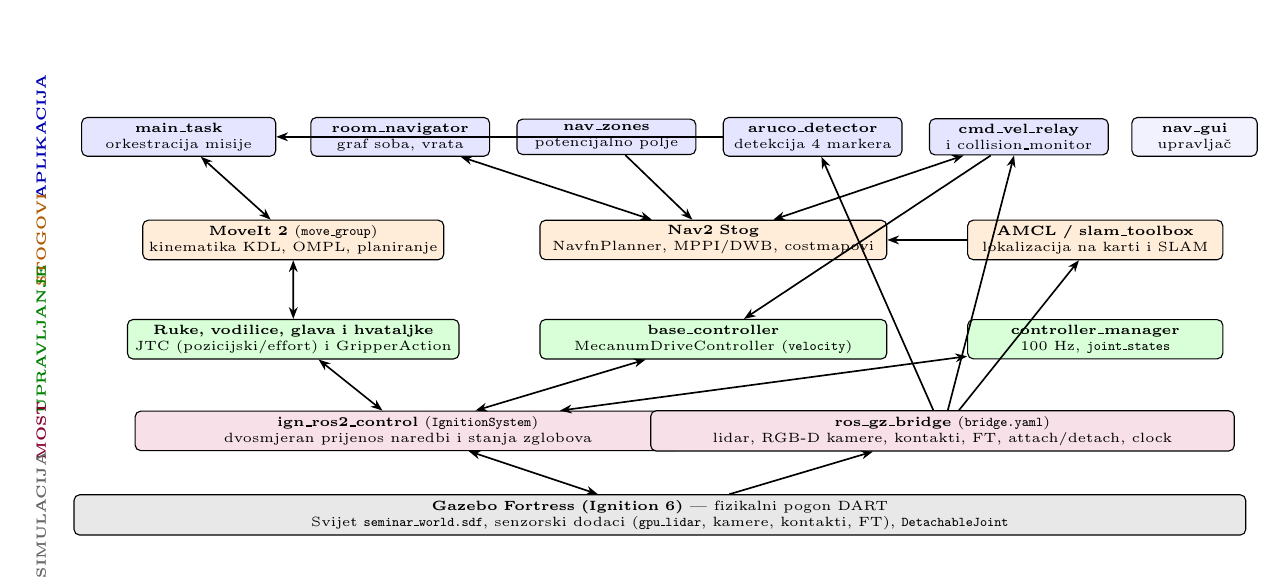
\begin{tikzpicture}[
  scale=0.97, transform shape,
  font=\scriptsize,
  layer/.style={draw, rounded corners=3pt, fill=#1, inner sep=4pt},
  nodebox/.style={draw, rounded corners=2pt, fill=white, align=center, inner sep=2pt, font=\tiny},
  arr/.style={-{Stealth[length=1.5mm]}, semithick},
  darr/.style={{Stealth[length=1.5mm]}-{Stealth[length=1.5mm]}, semithick}
]

  % Sloj 5: Aplikacija i misija (vrh)
  \begin{scope}[local bounding box=applayer]
    \node[nodebox, fill=blue!10, text width=24mm] (mt) at (1.5, 0) {\textbf{main\_task}\\orkestracija misije};
    \node[nodebox, fill=blue!10, text width=22mm] (rn) at (4.4, 0) {\textbf{room\_navigator}\\graf soba, vrata};
    \node[nodebox, fill=blue!10, text width=22mm] (nz) at (7.1, 0) {\textbf{nav\_zones}\\potencijalno polje};
    \node[nodebox, fill=blue!10, text width=22mm] (ad) at (9.8, 0) {\textbf{aruco\_detector}\\detekcija 4 markera};
    \node[nodebox, fill=blue!10, text width=22mm] (cm) at (12.5, 0) {\textbf{cmd\_vel\_relay}\\i collision\_monitor};
    \node[nodebox, fill=blue!5, text width=15mm] (gui) at (14.8, 0) {\textbf{nav\_gui}\\upravljač};
  \end{scope}

  % Sloj 4: Autonomni stogovi (MoveIt 2 & Nav2)
  \begin{scope}[local bounding box=stacklayer]
    \node[nodebox, fill=orange!15, text width=38mm] (moveit) at (3.0, -1.35)
      {\textbf{MoveIt 2} (\texttt{move\_group})\\kinematika KDL, OMPL, planiranje};
    \node[nodebox, fill=orange!15, text width=44mm] (nav2) at (8.5, -1.35)
      {\textbf{Nav2 Stog}\\NavfnPlanner, MPPI/DWB, costmapovi};
    \node[nodebox, fill=orange!15, text width=32mm] (amcl) at (13.5, -1.35)
      {\textbf{AMCL / slam\_toolbox}\\lokalizacija na karti i SLAM};
  \end{scope}

  % Sloj 3: ros2_control & Hardware Abstraction
  \begin{scope}[local bounding box=controllayer]
    \node[nodebox, fill=green!15, text width=42mm] (armctrl) at (3.0, -2.65)
      {\textbf{Ruke, vodilice, glava i hvataljke}\\JTC (pozicijski/effort) i GripperAction};
    \node[nodebox, fill=green!15, text width=44mm] (basectrl) at (8.5, -2.65)
      {\textbf{base\_controller}\\MecanumDriveController (\texttt{velocity})};
    \node[nodebox, fill=green!15, text width=32mm] (cmgr) at (13.5, -2.65)
      {\textbf{controller\_manager}\\100~Hz, \texttt{joint\_states}};
  \end{scope}

  % Sloj 2: Mostovi prema simulatoru
  \begin{scope}[local bounding box=bridgelayer]
    \node[nodebox, fill=purple!12, text width=70mm] (ignctrl) at (4.5, -3.85)
      {\textbf{ign\_ros2\_control} (\texttt{IgnitionSystem})\\dvosmjeran prijenos naredbi i stanja zglobova};
    \node[nodebox, fill=purple!12, text width=75mm] (gzbridge) at (11.5, -3.85)
      {\textbf{ros\_gz\_bridge} (\texttt{bridge.yaml})\\lidar, RGB-D kamere, kontakti, FT, attach/detach, clock};
  \end{scope}

  % Sloj 1: Gazebo simulator (dno)
  \begin{scope}[local bounding box=gzlayer]
    \node[nodebox, fill=gray!18, text width=152mm] (gzsim) at (7.8, -4.95)
      {\textbf{Gazebo Fortress (Ignition 6)} --- fizikalni pogon DART\\
       Svijet \texttt{seminar\_world.sdf}, senzorski dodaci (\texttt{gpu\_lidar}, kamere, kontakti, FT), \texttt{DetachableJoint}};
  \end{scope}

  % Oznake slojeva lijevo
  \node[font=\tiny\bfseries, text=blue!70!black, rotate=90] at (-0.3, 0) {APLIKACIJA};
  \node[font=\tiny\bfseries, text=orange!70!black, rotate=90] at (-0.3, -1.35) {STOGOVI};
  \node[font=\tiny\bfseries, text=green!50!black, rotate=90] at (-0.3, -2.65) {UPRAVLJANJE};
  \node[font=\tiny\bfseries, text=purple!70!black, rotate=90] at (-0.3, -3.85) {MOST};
  \node[font=\tiny\bfseries, text=gray!80!black, rotate=90] at (-0.3, -4.95) {SIMULACIJA};

  % Poveznice
  \draw[darr] (mt) -- (moveit);
  \draw[darr] (rn) -- (nav2);
  \draw[arr] (nz) -- (nav2);
  \draw[arr] (ad) -- (mt);
  \draw[arr] (cm) -- (basectrl);
  \draw[arr] (amcl) -- (nav2);
  \draw[darr] (moveit) -- (armctrl);
  \draw[darr] (nav2) -- (cm);
  \draw[darr] (armctrl) -- (ignctrl);
  \draw[darr] (basectrl) -- (ignctrl);
  \draw[darr] (cmgr) -- (ignctrl);
  \draw[darr] (ignctrl) -- (gzsim);
  \draw[arr] (gzsim) -- (gzbridge);
  \draw[arr] (gzbridge) -- (ad);
  \draw[arr] (gzbridge) -- (amcl);
  \draw[arr] (gzbridge) -- (cm);
\end{tikzpicture}

  \caption{Nacrt arhitekture sustava: pet slojeva od Gazebo fizike do aplikacijske orkestracije}
  \label{fig:arh-sustava}
\end{figure}

\subsection{Slojevi sustava i raspodjela čvorova}
\label{sec:02-slojevi}

% izvor: config/bridge.yaml:1-164; robot.urdf.xacro:479-481; launch/sim.launch.py:227-252
Simulacijski sloj izvodi se unutar simulatora Gazebo Fortress uz DART fizikalni rješavač.
Između Gazeba i ROS~2 ekosustava djeluju dva komplementarna mosta. Dodatak \texttt{ign\_ros2\_control}
\cite{mail2026} preko sučelja \texttt{IgnitionSystem} povezuje \texttt{controller\_manager}
s virtualnim zglobovima robota na frekvenciji od 100~Hz. Svi senzorski tokovi (lidar, RGB-D kamere,
kontaktni senzori na prstima, dvoosni tenzometrijski FT senzori) te naredbe za kruto spajanje
kocke (\texttt{DetachableJoint}) prenose se putem paketa \texttt{ros\_gz\_bridge} prema
deklaraciji u \texttt{bridge.yaml}.

% izvor: pas_dual_arm_scripts/setup.py:28-44; main_task.py; room_navigator.py; nav_zones.py
U tablici~\ref{tab:cvorovi} prikazani su ključni aplikacijski čvorovi razvijeni u sklopu paketa
\texttt{pas\_dual\_arm\_scripts}, njihove primarne odgovornosti te ulazno-izlazna komunikacijska sučelja.

\begin{table}[H]
  \centering
  \scriptsize
  \setstretch{1.05}
  \caption{Pregled aplikacijskih čvorova sustava u paketu \texttt{pas\_dual\_arm\_scripts}}
  \label{tab:cvorovi}
  \begin{tabularx}{\textwidth}{@{}>{\bfseries}p{2.8cm}>{\raggedright\arraybackslash}X>{\raggedright\arraybackslash}p{4.6cm}@{}}
    \toprule
    Čvor & Glavna odgovornost & Ključne teme, akcije i servisi \\
    \midrule
    \texttt{main\_task} & Orkestracija misije (8 koraka), dvoručni hvat, vizualno navođenje, odlaganje & Ulaz: \texttt{/mission/start}, detekcije, TF\newline Izlaz: \texttt{/room\_navigator/goto}, akcije ruku \\
    \texttt{room\_navigator} & Navigacija među sobama, prolazak kroz vrata uz provjeru poze ruku & Ulaz: \texttt{/room\_navigator/goto}, \texttt{/joint\_states}\newline Izlaz: \texttt{/navigate\_through\_poses}, status \\
    \texttt{nav\_zones} & Izračun jedinstvenog potencijalnog polja i brazdi nulte cijene iz karte & Ulaz: \texttt{/map}\newline Izlaz: \texttt{/nav\_zones/field} (costmap filter) \\
    \texttt{feature\_registry} & Semantičko prepoznavanje vrata, stolova i dock poza iz geometrije & Ulaz: \texttt{/map}\newline Izlaz: registar značajki, servisi koordinata \\
    \texttt{aruco\_detector} & Detekcija ArUco markera (glava i zapešća), estimacija 6D poze & Ulaz: \texttt{/camera/*}, \texttt{/wrist\_*/*}\newline Izlaz: \texttt{/aruco\_detections}, objave u \texttt{/tf} \\
    \texttt{cmd\_vel\_relay} & Arbitraža i sigurnosno prespajanje brzinskih naredbi baze & Ulaz: \texttt{/cmd\_vel\_safe}, \texttt{/cmd\_vel}\newline Izlaz: \texttt{reference\_unstamped} \\
    \texttt{collision\_monitor} & Neposredno zaustavljanje baze na temelju laserskog obrisa & Ulaz: \texttt{/scan\_filtered}, poligon obrisa\newline Izlaz: \texttt{/cmd\_vel\_safe} \\
    \texttt{footprint\_publisher} & Dinamičko prilagođavanje tlocrtnog poligona robota i nošene kocke & Ulaz: stanje misije, \texttt{/joint\_states}\newline Izlaz: \texttt{/footprint}, \texttt{/mission/carried\_points} \\
    \texttt{scan\_filter} & Uklanjanje točaka vlastitog tijela i kotača iz laserskog skena & Ulaz: \texttt{/scan}\newline Izlaz: \texttt{/scan\_filtered} \\
    \texttt{nav\_gui} & Tkinter grafičko sučelje za praćenje misije i ručni start & Ulaz: \texttt{/mission/task\_status}\newline Izlaz: objava na \texttt{/mission/start} \\
    \bottomrule
  \end{tabularx}
\end{table}

\subsection{Koordinatni sustavi i stablo transformacija (TF)}
\label{sec:02-tf}

% izvor: robot.urdf.xacro:20-250; kortex .../gen3.xacro; base.urdf.xacro; pan_tilt.xacro
Prostorni odnosi i kinematičke veze formalizirani su kroz stablo transformacija okvira (\texttt{/tf}
i \texttt{/tf\_static}). Ishodište navigacijskog prostora čini globalni okvir \texttt{map}, u kojem
algoritam AMCL procjenjuje pozu odometrijskog okvira \texttt{odom}. Kontroler baze
\texttt{mecanum\_drive\_controller} putem releja \texttt{cmd\_vel\_relay} objavljuje transformaciju
između \texttt{odom} i tlocrtne projekcije robota \texttt{base\_footprint}, na koju se nadovezuje
strukturna točka \texttt{base\_link}.

Kinematičko stablo robota grana se iz okvira \texttt{base\_link} na četiri glavne grane:
\begin{enumerate}
  \item \textbf{Lidar}: \texttt{base\_link} $\rightarrow$ \texttt{laser\_link} (postavljen na visini $0{,}209$~m, usmjeren vodoravno prema naprijed).
  \item \textbf{Torzo i vodilice}: \texttt{base\_link} $\rightarrow$ \texttt{torso\_link} $\rightarrow$ prizmatični zglobovi $\rightarrow$ klizači \texttt{torso\_left\_carriage\_link} i \texttt{torso\_right\_carriage\_link}.
  \item \textbf{Robotske ruke i hvataljke}: sa svakog klizača grana se kinematički lanac Kinova Gen3 manipulatora (\texttt{*\_base\_link} $\rightarrow$ zglobovi $1\dots7$ $\rightarrow$ \texttt{*\_end\_effector\_link} $\rightarrow$ \texttt{*\_bracelet\_link}), na koji su montirane kamere zapešća (\texttt{wrist\_*\_camera\_link}) te baze hvataljki Robotiq 2F-85 s kinematikom prstiju.
  \item \textbf{Pan-tilt glava}: s vrha torza (\texttt{torso\_link}) lanac vodi preko rotacijskih zglobova \texttt{pan\_tilt\_yaw\_link} i \texttt{pan\_tilt\_pitch\_link} do optičkog okvira RGB-D kamere \texttt{camera\_color\_optical\_frame}.
\end{enumerate}
Detektirani ArUco markeri i manipulirana kocka dinamički se vežu u TF stablo preko okvira kamere koja
ih trenutno opaža (\texttt{camera\_link} ili \texttt{wrist\_*\_link}), dok čvor \texttt{main\_task}
prilikom hvata pamti fiksnu transformaciju kocke u odnosu na zapešće (\texttt{\_hold}) kako bi
očuvao praćenje objekta kada marker izađe iz vidnog polja.

\subsection{Hijerarhija pokretačkih skripti (Launch)}
\label{sec:02-launch}

% izvor: launch/mission.launch.py:1-107; launch/sim.launch.py; launch/nav2.launch.py; launch/task.launch.py
Pokretanje cjelokupnog sustava izvedeno je hijerarhijski kroz četiri ugniježđene pokretačke skripte
(slika~\ref{fig:launch-hijerarhija}). Krovna datoteka \texttt{mission.launch.py} uvodi precizno
odmjerena vremenska kašnjenja kako bi se spriječilo zagušenje procesora i osigurala dostupnost
ROS~2 servisa prije pokretanja ovisnih čvorova:

\begin{figure}[H]
  \centering
  % G05: Hijerarhija pokretackih datoteka (mission.launch.py -> sim, nav2, task)
% Izvori: launch/mission.launch.py:20-107, launch/sim.launch.py, launch/nav2.launch.py, launch/task.launch.py
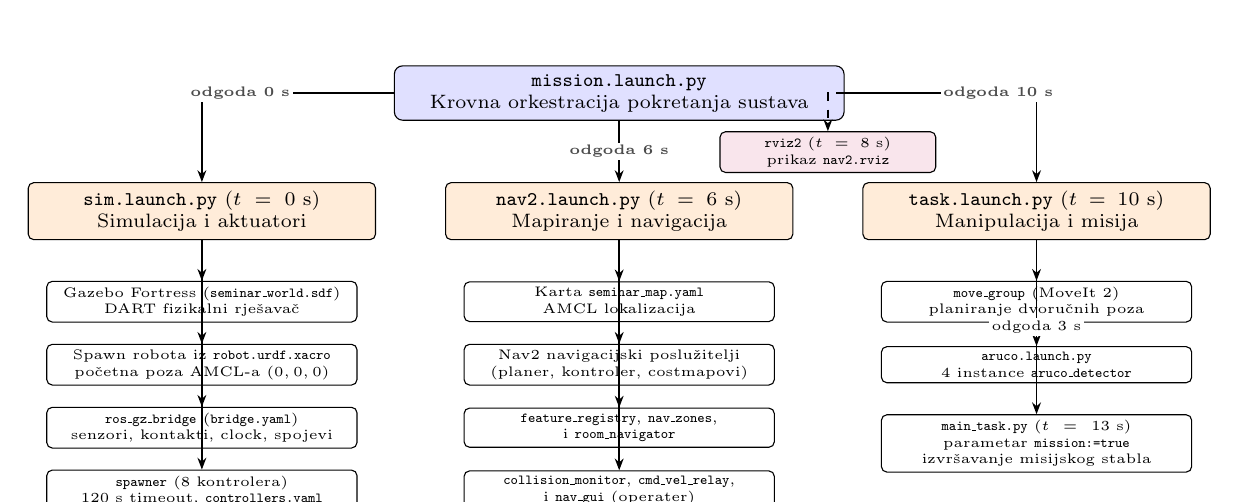
\begin{tikzpicture}[
  font=\scriptsize,
  topl/.style={draw, rounded corners=3pt, fill=blue!12, align=center, text width=55mm, inner sep=3pt},
  subl/.style={draw, rounded corners=2pt, fill=orange!15, align=center, text width=42mm, inner sep=3pt},
  nodebox/.style={draw, rounded corners=2pt, fill=white, align=center, text width=38mm, inner sep=2pt, font=\tiny},
  arr/.style={-{Stealth[length=1.5mm]}, semithick},
  lbl/.style={font=\tiny\bfseries, text=black!70, fill=white, inner sep=1pt}
]

  % Vrh: mission.launch.py
  \node[topl] (mission) at (7.5, 0)
    {\textbf{\texttt{mission.launch.py}}\\Krovna orkestracija pokretanja sustava};

  % Podređeni launch fajlovi
  \node[subl] (sim) at (2.2, -1.5)
    {\textbf{\texttt{sim.launch.py}} ($t = 0$~s)\\Simulacija i aktuatori};
  \node[subl] (nav) at (7.5, -1.5)
    {\textbf{\texttt{nav2.launch.py}} ($t = 6$~s)\\Mapiranje i navigacija};
  \node[subl] (task) at (12.8, -1.5)
    {\textbf{\texttt{task.launch.py}} ($t = 10$~s)\\Manipulacija i misija};

  % RViz (t = 8 s)
  \node[nodebox, fill=purple!10, text width=26mm] (rviz) at (10.15, -0.75)
    {\textbf{\texttt{rviz2}} ($t = 8$~s)\\prikaz \texttt{nav2.rviz}};

  % Čvorovi pod sim
  \node[nodebox] (gz) at (2.2, -2.65)
    {Gazebo Fortress (\texttt{seminar\_world.sdf})\\DART fizikalni rješavač};
  \node[nodebox] (spwn) at (2.2, -3.45)
    {Spawn robota iz \texttt{robot.urdf.xacro}\\početna poza AMCL-a $(0,0,0)$};
  \node[nodebox] (bridge) at (2.2, -4.25)
    {\texttt{ros\_gz\_bridge} (\texttt{bridge.yaml})\\senzori, kontakti, clock, spojevi};
  \node[nodebox] (ctrl) at (2.2, -5.05)
    {\texttt{spawner} (8 kontrolera)\\120~s timeout, \texttt{controllers.yaml}};

  % Čvorovi pod nav2
  \node[nodebox] (amclnode) at (7.5, -2.65)
    {Karta \texttt{seminar\_map.yaml}\\AMCL lokalizacija};
  \node[nodebox] (navstack) at (7.5, -3.45)
    {Nav2 navigacijski poslužitelji\\(planer, kontroler, costmapovi)};
  \node[nodebox] (navhelper) at (7.5, -4.25)
    {\texttt{feature\_registry}, \texttt{nav\_zones},\\i \texttt{room\_navigator}};
  \node[nodebox] (navsafety) at (7.5, -5.05)
    {\texttt{collision\_monitor}, \texttt{cmd\_vel\_relay},\\i \texttt{nav\_gui} (operater)};

  % Čvorovi pod task
  \node[nodebox] (mg) at (12.8, -2.65)
    {\texttt{move\_group} (MoveIt~2)\\planiranje dvoručnih poza};
  \node[nodebox] (aruco) at (12.8, -3.45)
    {\texttt{aruco.launch.py}\\4 instance \texttt{aruco\_detector}};
  \node[nodebox] (mtask) at (12.8, -4.45)
    {\textbf{\texttt{main\_task.py}} ($t = 13$~s)\\parametar \texttt{mission:=true}\\izvršavanje misijskog stabla};

  % Poveznice
  \draw[arr] (mission) -| node[lbl, pos=0.4] {odgoda 0~s} (sim);
  \draw[arr] (mission) -- node[lbl] {odgoda 6~s} (nav);
  \draw[arr] (mission) -| node[lbl, pos=0.4] {odgoda 10~s} (task);
  \draw[arr, dashed] (mission) -| (rviz);

  \draw[arr] (sim) -- (gz);
  \draw[arr] (sim) -- (spwn);
  \draw[arr] (sim) -- (bridge);
  \draw[arr] (sim) -- (ctrl);

  \draw[arr] (nav) -- (amclnode);
  \draw[arr] (nav) -- (navstack);
  \draw[arr] (nav) -- (navhelper);
  \draw[arr] (nav) -- (navsafety);

  \draw[arr] (task) -- (mg);
  \draw[arr] (task) -- (aruco);
  \draw[arr] (task) -- node[font=\tiny, fill=white, inner sep=1pt] {odgoda 3~s} (mtask);
\end{tikzpicture}

  \caption{Hijerarhijski slijed pokretačkih skripti s vremenskim razmacima inicijalizacije}
  \label{fig:launch-hijerarhija}
\end{figure}

U trenutku $t = 0$~s \texttt{sim.launch.py} pokreće simulator Gazebo, učitava URDF model preko
xacro procesora, stvara robota u ishodištu svijeta (početna AMCL poza $(0, 0, 0)$), uspostavlja
\texttt{ros\_gz\_bridge} te pokreće spawner procese za svih osam kontrolera s rokom čekanja od 120~s.
Nakon 6~s \texttt{nav2.launch.py} podiže kartu, AMCL lokalizaciju, Nav2 poslužitelje, potencijalna
polja i sigurnosne monitore. U trenutku $t = 8$~s opcionalno se otvara RViz2, a na $t = 10$~s
\texttt{task.launch.py} aktivira \texttt{move\_group} i detektore markera. Konačno, na $t = 13$~s
pokreće se \texttt{main\_task} s argumentom \texttt{mission:=true}, čime započinje autonomna misija.

\subsection{Struktura repozitorija, ovisnosti i projektno okruženje}
\label{sec:02-repozitorij}

% izvor: ros2.repos:1-35; patches/*; scripts/run_native.sh; README.md §8-9
Izvorni kod projekta podijeljen je u četiri vlastita paketa unutar direktorija \texttt{src/}:
\begin{itemize}
  \item \texttt{pas\_dual\_arm\_bringup}: pokretačke skripte cijelog sustava, konfiguracijske YAML datoteke za kontrolere, Nav2 i mostove, te definicija simulacijskog svijeta i karata.
  \item \texttt{pas\_dual\_arm\_scripts}: implementacija svih misijskih, navigacijskih i percepcijskih čvorova u programskom jeziku Python.
  \item \texttt{pas\_dual\_arm\_description}: cjeloviti xacro modeli sklopljenog robota, omnidirekcijske baze, senzorskih elemenata i kolizijskih geometrija.
  \item \texttt{pas\_dual\_arm\_moveit\_config}: semantički opisi robota (SRDF), konfiguracija kinematičkih rješavača KDL i OMPL algoritama za dvoručni sustav.
  \item \texttt{dual\_arm\_torso}: CAD meshevi i kinematički opis linearnih vodilica torza \cite{mail2026}.
\end{itemize}

% izvor: ros2.repos:20-35; patches/
Vanjski paketi definirani su u datoteci \texttt{ros2.repos} i vezani na točno određene commitove:
\texttt{ros2\_kortex} (\texttt{116d87a}), \texttt{omni\_base\_simulation} (\texttt{77248ac}),
\texttt{pan\_tilt\_ros} (\texttt{9b08758}), \texttt{realsense-ros} (\texttt{6d87b07}) i
\texttt{aruco\_ros} (\texttt{86a0bbb}). Nad vanjskim paketima primijenjene su dvije lokalne
zakrpe u direktoriju \texttt{patches/}: \texttt{pan\_tilt\_ros} zakrpa koja dodaje korektne inercijske
matrice i granice momenta za Gazebo Fortress fiziku te zakrpa za \texttt{ros2\_kortex} koja uklanja
nepodržane Isaac Gym argumente iz makroa Robotiq 2F-85 hvataljke.

% izvor: scripts/run_native.sh; notes/03_problemi/P-01_shell_zenoh_contamination.md
Za pouzdano i determinističko izvođenje razvijena je skripta \texttt{./scripts/run\_native.sh}, koja
postavlja izoliranu okolinu, definira \texttt{RMW\_IMPLEMENTATION=rmw\_cyclonedds\_cpp} i
\texttt{IGN\_GAZEBO\_RESOURCE\_PATH} te sprječava interferenciju sa sustavskim varijablama i vanjskim
middleware protokolima (npr. Zenoh, zabilježen u problemu P-01).

\section{Model robota i simulacijsko okruženje}
\label{sec:03-model-i-okruzenje}

\section{Upravljanje sustavom (ros2\_control)}
\label{sec:04-upravljanje}

\section{Percepcija}
\label{sec:05-percepcija}

\section{Mapiranje i navigacija}
\label{sec:06-navigacija}

\section{Manipulacija i dvoručni hvat}
\label{sec:07-manipulacija}

\section{Orkestracija misije}
\label{sec:08-misija}

\section{Rezultati, problemi i ograničenja}
\label{sec:09-rezultati}

% izvor: notes/05_povijest/runovi.md; notes/00_MAPA.md; notes/03_problemi/*; README.md §10
U ovom poglavlju sažeti su kvantitativni eksperimentalni rezultati autonomne misije, analizirani
ključni inženjerski problemi razriješeni tijekom razvoja te dokumentirana stvarna fizikalna i
softverska ograničenja sustava u skladu s načelom inženjerske iskrenosti (odluka D-12).

\subsection{Eksperimentalno izmjereni rezultati}
\label{sec:09-mjerenja}

% izvor: runovi.md (runovi 44, 60, 62, 70, M1, M4, T2); scripts/check_*.py
Verifikacija sustava provedena je kroz seriju ciljanih pokusa u simulacijskom okruženju Gazebo
Fortress. U tablici~\ref{tab:rezultati} prikazani su ključni izmjereni pokazatelji navigacijske,
percepcijske i manipulacijske uspješnosti.

\begin{table}[H]
  \centering
  \scriptsize
  \setstretch{1.05}
  \caption{Kvantitativni rezultati ključnih verifikacijskih pokusa i misijskih ciklusa}
  \label{tab:rezultati}
  \begin{tabularx}{\textwidth}{@{}>{\bfseries}p{1.8cm}>{\raggedright\arraybackslash}p{2.8cm}>{\raggedright\arraybackslash}X>{\raggedright\arraybackslash}p{3.2cm}@{}}
    \toprule
    Pokus / Run & Ispitivani podsustav & Izmjereni pokazatelji i tolerancije & Ishod i status \\
    \midrule
    Karta (run~60) & SLAM lasersko mapiranje (\texttt{slam\_toolbox}) & Otvor vrata $0{,}980$~m (nominalno $1{,}0$~m); os $0{,}0$~cm; debljina zida $120$~mm; RMS lica $\le \SI{2.3}{mm}$ & Prihvaćena finalna karta (\texttt{check\_map\_geometry}) \\
    Lokalizacija (run~62) & AMCL probabilistička lokalizacija & $5/5$ prolaza kroz vrata bez prekida; vršna greška AMCL vs Gazebo $3{,}0$~cm ($X$), $2{,}9$~cm ($Y$), $0{,}3^\circ$ (yaw) & Validiran mjerni model (\texttt{loc\_error.py}) \\
    Navigacija (run~70) & Potencijalna polja (odluka D-20) & Puni obilazak obaju stolova; razmak od prepreka $0{,}715$~m; uspješan dock i 1D undock & Potvrđeno kretanje bez kolizija i zastoja \\
    Vožnja (run~M1) & Transportna poza ruku \texttt{DRIVE\_V4} & 9 zadanih ciljeva; 3 uzastopna prolaska kroz vrata; odstupanje ruku $0{,}000$~rad; bočni zazor $4{,}4$--$4{,}9$~cm & Validiran kinematički profil vožnje baze \\
    Misija (run~M4) & Puni autonomni ciklus (jedna naredba) & Dvoručni hvat i dizanje na $0{,}55$~m; nošenje u \texttt{CARRY\_V4} ($0{,}821$~m); spuštanje na $+4$~mm od ploče stola & \texttt{PLACE VERIFIED: 5 mm} od centra; \texttt{MISSION COMPLETE} \\
    Build (run~T2) & Reproducibilnost čistog repozitorija & $25/25$ paketa uspješno izgrađeno iz nule (\texttt{vcs import} uz zakrpe); 17/17 sistemskih provjera prolazi & Potvrđena prenosivost na čistim instalacijama \\
    \bottomrule
  \end{tabularx}
\end{table}

\subsection{Pregled ključnih problema i rješenja}
\label{sec:09-problemi}

% izvor: notes/03_problemi/P-09, P-13, P-15, P-17, P-35, P-39, P-40, P-43, P-45, P-46
Razvoj autonomnog mobilnog manipulatora zahtijevao je rješavanje niza složenih problema
uzrokovanih numeričkim nesavršenostima simulatora, geometrijom kinematičkih lanaca i međuovisnostima
heterogenih ROS~2 paketa. U tablici~\ref{tab:problemi} sažeti su ključni problemi, njihovi fizikalni
i programski uzroci te implementirana rješenja.

\begin{table}[H]
  \centering
  \scriptsize
  \setstretch{1.05}
  \caption{Pregled ključnih inženjerskih problema riješenih tijekom razvoja sustava}
  \label{tab:problemi}
  \begin{tabularx}{\textwidth}{@{}>{\bfseries}p{1.4cm}>{\raggedright\arraybackslash}p{3.2cm}>{\raggedright\arraybackslash}X>{\raggedright\arraybackslash}X@{}}
    \toprule
    Problem & Simptom i manifestacija & Fizikalni ili programski uzrok & Implementirano rješenje \\
    \midrule
    P-09 & Izostanak bočnog gibanja baze u Gazebu Fortress & PAL kontroler pisan za Gazebo Classic; Fortress dodaci se ne instanciraju & Konfiguriran \texttt{MecanumDriveController} uz valjkastu koliziju i anizotropno trenje kotača \\
    P-13 & Linearne vodilice torza ne podižu teret ruku & Donji položaj ($0{,}05$~m) na graničniku gdje dodatak poništava brzinu & Postavljen početni položaj klizača na $0{,}06$~m (\texttt{initial\_value}) \\
    P-15 & Kocka isklizava iz šaka prilikom dizanja & DART kontaktni rješavač u Fortressu ne drži statičko trenje pod stiskom & Uveden \texttt{DetachableJoint} uz obaveznu fizikalnu provjeru dodira senzora (D-05, D-12) \\
    P-17 & Nestabilnost simulacije (eksplozija kocke u zrak) & Dvostruka kruta kinematička veza i aktivni IK čine preodređen sustav & Jednostrani spoj na lijevoj šaci; desni jastučić popušta $2$~mm i ostaje u kontaktu (D-07) \\
    P-35, P-43 & Širina ruku veća od otvora vrata ($1{,}003 > 0{,}980$~m) & Vodoravni prilaz postavlja sferna zapešća u poprečnu liniju maksimalnog raspona & Prilaz pod nagibom od $55^\circ$ prema dolje (\texttt{GRASP\_V4}) i poza nošenja \texttt{CARRY\_V4} ($0{,}821$~m) \\
    P-39 & Robot ulazi u vrata pod kutom i zapinje za dovratnik & NavFn planira točku bez orijentacije; filtar lidara brisao dovratnike & Usmjeravajuće trake u \texttt{nav\_zones}, sužen filtar na $0{,}30$~m, brazde nulte cijene \\
    P-40 & AMCL procjena poze odstupa od lidara za 6~cm & Gruba rešetka karte ($0{,}05$~m) umjetno podebljala zidove na $178$~mm & Karta rešetke $0{,}02$~m s 1080 zraka lidara i podešenim \texttt{likelihood\_field} modelom \\
    P-45 & Misija staje pred stolom ili gubi naredbu odvajanja & Latched statusi navigacije i gubitak poruke \texttt{ign topic} bez potvrde & Stanja u zatvorenoj petlji; dvostruki ROS/Ignition most za detach uz provjeru \texttt{/aruco\_box/state} \\
    P-46 & Čisti klon s GitHuba ne prolazi proces izgradnje & U \texttt{ros2.repos} greškom upisan lokalni neprenosivi commit & Pinani stvarni upstream commitovi uz lokalne zakrpe u direktoriju \texttt{patches/} \\
    \bottomrule
  \end{tabularx}
\end{table}

\subsection{Identificirana ograničenja sustava}
\label{sec:09-ogranicenja}

% izvor: notes/03_problemi/*; notes/07_predaja/odstupanja.md; README.md §10
Iako je cjelovita misija uspješno demonstrirana u simulaciji, sustav posjeduje određena
ograničenja koja valja uzeti u obzir:
\begin{enumerate}
  \item \textbf{Ograničenje trenja fizikalnog rješavača}: Podizanje tereta oslanja se na dodatak
    \texttt{DetachableJoint} jer DART fizikalni pogon u Gazebo Fortressu ne može pouzdano simulirati
    suho Coulombovo trenje između paralelnih ploha pod dinamičkim opterećenjem bez proklizavanja.
  \item \textbf{Osjetljivost percepcije na kut promatranja}: Detekcija ArUco markera kamerom glave
    postaje nepouzdana pri udaljenostima manjim od $\SI{0.60}{m}$ zbog oštrog kuta skraćenja, što je
    zahtijevalo uvođenje dodatnih kamera na zapešćima ruku.
  \item \textbf{Fiksna geometrija manipulacijskog objekta}: Sustav je dimenzioniran i provjeren za
    kocku brida $\SI{0.30}{m}$. Manipulacija objektima znatno različitih dimenzija ili nepravilnih
    oblika zahtijevala bi prilagodbu kinematičkih konfiguracija i pragova geometrijskih filtara.
  \item \textbf{Numerička zahtjevnost simulacije}: Zbog istodobnog izvođenja fizike krutih tijela,
    kontaktne dinamike, obrade četiriju kamera, simulacije 1080 zraka lidara te rada stogova MoveIt~2
    i Nav2, sustav zahtijeva značajne računalne resurse kako faktor realnog vremena (RTF) ne bi pao
    ispod stabilne radne točke.
\end{enumerate}

\section{Zaključak}
\label{sec:zakljucak}

% izvor: notes/00_MAPA.md; notes/05_povijest/runovi.md; README.md §10
U okviru ovog rada uspješno je projektiran, modeliran i verificiran cjeloviti simulacijski model
dvoručnog mobilnog manipulatora PAS-DUAL-ARM u okruženju Gazebo Fortress i ROS~2 Humble, u skladu sa
svim zahtjevima kolegija \emph{Projektiranje autonomnih sustava} \cite{zadatak2025, mail2026}.

Integracijom omnidirekcijske mobilne baze, torza s dvjema linearnim vodilicama, dviju robotskih ruku
Kinova Gen3 s hvataljkama Robotiq 2F-85 te pan-tilt glave s RGB-D kamerom ostvaren je složen
kinematički i dinamički sustav s ukupno 24 upravljana zgloba. Sustav je u potpunosti objedinjen unutar
okvira \texttt{ros2\_control} uz frekvenciju rada od 100~Hz.

Autonomna misija preuzimanja i transporta manipulacijske kocke uspješno je demonstrirana iz jedne
pokretačke naredbe (\texttt{mission.launch.py}):
\begin{enumerate}
  \item \textbf{Precizno lasersko mapiranje i navigacija}: Korištenjem paketa \texttt{slam\_toolbox}
    i lidara s 1080 zraka na rešetki od $\SI{0.02}{m}$ generirana je geometrijski egzaktna karta s
    izmjereno čistim otvorom vrata od $0{,}980$~m. Uvođenjem jedinstvenog potencijalnog polja s
    usmjeravajućim trakama kroz vrata i nultim brazdama (\texttt{nav\_zones.py}) riješen je problem
    kosog ulaska u vrata, čime je omogućen siguran prolazak robota sa samo $6{,}3$~cm bočnog zazora.
  \item \textbf{Pouzdana dvoručna manipulacija}: Zbog geometrijskih ograničenja sfernog zapešća
    razvijena je nagnuta poza hvata (\texttt{GRASP\_V4}, nagib $55^\circ$ prema dolje) i poza nošenja
    (\texttt{CARRY\_V4}, širina $0{,}821$~m), što je omogućilo prolazak s teretom kroz vrata. Hvat se
    potvrđuje očitanjima kontaktnih senzora na prstima ruku prije aktivacije dodatka
    \texttt{DetachableJoint}, čime je zadovoljeno načelo poštene verifikacije bez lažnog hvata.
  \item \textbf{Milimetarska točnost odlaganja}: Slijed odlaganja kocke u 11 koraka
    (\texttt{main\_task.py}) vodi robot i manipulator pomoću vizualne detekcije ciljnog markera ID~3
    te završava spuštanjem na visinu od $+4$~mm iznad stola i verificiranim odstupanjem središta od
    samo $\SI{5}{mm}$ od centra markera.
\end{enumerate}

Ključna inženjerska lekcija proizašla iz ovog projekta jest nužnost uvođenja zatvorenih petlji
provjere: u složenom simulacijskom okruženju status akcije (npr. \texttt{SUCCEEDED}) ne jamči da je
aktuator pod opterećenjem doista dosegao ciljni položaj. Verifikacija stvarnih kutova zglobova,
prostornih transformacija iz TF stabla i stanja fizikalnih senzora prije svakog kritičnog prijelaza
omogućila je determinističko i robusno izvršavanje misije od početka do kraja.


% ---- LITERATURA ----
\clearpage
\bibliographystyle{unsrt}
\bibliography{references}

% ---- PRILOZI (iza literature) ----
\clearpage
\appendix
\section{Pokretanje sustava}
\label{sec:prilog-a-pokretanje}

\section{Izvodi iz koda}
\label{sec:prilog-b-kod}


\end{document}
